\documentclass[12pt, french]{article}

\usepackage{fancyhdr, fancybox, lastpage}
\usepackage[most]{tcolorbox}
\usepackage[a4paper, margin={0.3in, .75in}]{geometry}
\usepackage{wrapfig}
\pagestyle{fancy}
\renewcommand\headrulewidth{1pt}
\renewcommand\footrulewidth{1pt}
\fancyhf{}
\rhead{ \em{Zakaria Haouzan}}
\lhead[C]{\em{Tronc Commun scientifique - option français (TCSBiof)}}
\chead[C]{}
\rfoot[C]{}
\lfoot[R]{}
\cfoot[]{\em{Page \thepage / \pageref{LastPage}}}


\newtcolorbox{Box2}[2][
enhanced, 
    breakable,
]{
                lower separated=false,
                colback=white,
colframe=white!20!black,fonttitle=\bfseries,
colbacktitle=white!30!gray,
coltitle=black,
enhanced,
attach boxed title to top left={yshift=-0.1in,xshift=0.15in},
title=#2,#1}


\begin{document}
\begin{center}
   \shadowbox {\bf{concentration molaire des espèces moléculaires dans une solution}}
\end{center}
\begin{center}
   \Large{ \em{Exercices Supplémentaires}}
\end{center}

%%_________________________Exercice ! :"_________________________Exercice
   \begin{Box2}{Exercice 1 : La phénolphtaléine }

%\begin{wrapfigure}[2]{r}{0.22\textwidth}
  %\begin{center}
	%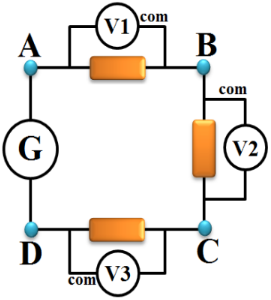
\includegraphics[width=0.22\textwidth]{./img/ex00.png}
  %\end{center}
%\end{wrapfigure}

	   La phénolphtaléine est un indicateur coloré acido-basique de formule $C_{20}H_{14}O_4$. Elle est utilisée en
	   solution dans l’éthanol à la concentration $C=1,3.10^{-3}mol.L^{-1}$
.

\begin{enumerate}
	\item Quel est le solvant de cette solution.
	\item  Quelle quantité de phénolphtaléine doit être utilisée pour préparer 250mL de cette solution
alcoolique.
\item  quelle est la masse de phénolphtaléine correspondante.
\end{enumerate}
	Données:
masses molaires en g/mol : M(H) = 1,0; M(C) = 12,0; M(O) = 16,0.

   \end{Box2}


%%_________________________Exercice !2 :"_________________________Exercice
\begin{Box2}{Exercice 2 :dilution d'une solution d'antiseptique}
Le Ramet de Dalibour est une solution contenant, entre autres, du sulfate de cuivre II à la concentration de $C_1=6,3.10^{-3}mol.L^{-1}$. et du sulfate de zinc à la concentration $C_2=2,17.10^{-2} mol.L^{-1}$ . En dermatologie, elle est utilisée pure ou diluée 2 fois.

\begin{enumerate}
\item Dans ce dernier cas quel est la valeur du facteur de dilution?
\item  Quelles sont alors les concentrations en sulfate de cuivre II et en sulfate de zinc de
la solution diluée?
\item  Décrire la préparation par dilution d’un volume V’= 100mL de cette solution diluée.
\end{enumerate}
   % \begin{wrapfigure}[2]{r}{0.2\textwidth}
  %\begin{center}
	  %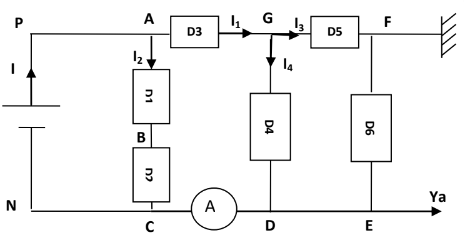
\includegraphics[width=0.2\textwidth]{./img/ex01.png}
  %\end{center}
%\end{wrapfigure}

\end{Box2}

%%_________________________Exercice ! 3:"_________________________Exercice
\begin{Box2}{Exercice 3 :l'eau de Javelle  }
   % \begin{wrapfigure}[2]{r}{0.25\textwidth}
  %\begin{center}
	%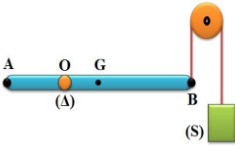
\includegraphics[width=0.25\textwidth]{./img/ex02.png}
  %\end{center}
%\end{wrapfigure}
	\begin{enumerate}
		\item Un consommateur a acheté une bouteille de Javelle d'un volume de V1=250mL, et avant de l'utiliser, il
verse-là dans un flacon de volume V2=1L, puis il remplit le flacon avec de l'eau. Calculer la valeur du coefficient de dilution.

\item Nous voulons diluer la solution de chlorure de sodium trois fois (soit au tiers de sa concentration
initiale). Nous avons pris un échantillon de cette solution de volume V1 =150mL.Calculer le volume d'eau distillée Veau qui doit être ajouté à cet échantillon pour faire cette dilution.
\end{enumerate}

\end{Box2}



%%_________________________Exercice 4 : _________________________Exercice
\begin{Box2}{Exercice 4 :la concentration molaire d'une solution commerciale}
L’étiquette de la solution commerciale d'ammoniac porte les indications suivantes:

 - Densité d = 0,95.
 
 - Le pourcentage massique d'ammoniac est $P = 28 \%$.

 \begin{enumerate}
	 \item Montrer que la concentration C0 de la solution commerciale s'écrit sous la forme : $C_0 = \frac{P.d.\rho_{eau}}{100.M}$
	 \item calculer $C_0$.
	 \item Déterminer le volume $V_0$ à prélever de la solution commerciale pour préparer $V_1=500mL$ d’une solution diluée de concentration $C_1=0,1mol/L$.
\item Calculer le facteur de dilution.

Données: La masse molaire de l'ammoniac: $M(NH_3) = 17 g/mol$.

 \end{enumerate}
   % \begin{wrapfigure}[1]{r}{0.28\textwidth}
		%\vspace{-0.5cm}
  %\begin{center}
	%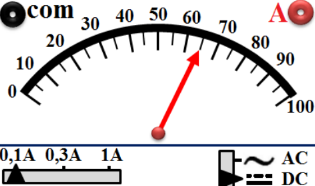
\includegraphics[width=0.28\textwidth]{./img/ex04.png}
  %\end{center}
%\end{wrapfigure}


\end{Box2}


%%_________________________Exercice 5 : _________________________Exercice
\begin{Box2}{Exercice 5 :la concentration C d'une solution commerciale d'un flacon de déboucheur }
   % \begin{wrapfigure}{r}{0.25\textwidth}
  %\end{wrapfigure}
Un flacon de déboucheur pour évier porte les indications suivantes: "Produit corrosif; Contient de l’hydroxyde de sodium (soude caustique); Solution à 20\%; La densité du produit est d=1,2".

Le pourcentage indiqué représente le pourcentage massique d’hydroxyde de sodium (NaOH) contenu
dans le produit.
\begin{enumerate}
\item Calculer la masse d’hydroxyde de sodium contenu dans 500 mL de produit.
\item  En déduire la concentration $C_0$ en soluté hydroxyde de sodium de la solution commerciale.
\item  On désire préparer un volume $V_1$ de solution $S_1$ de déboucheur 20 fois moins concentré que la
solution commerciale.
\begin{enumerate}
\item Quelle est la valeur de la concentration $C_1$ de la solution ?
\item Quelle est la quantité de matière d’hydroxyde de sodium contenu dans 250 mL de solution $S_1$?
\item Quel volume de solution commerciale a-t-il fallu prélever pour avoir cette quantité de matière
d’hydroxyde de sodium?
\end{enumerate}
\end{enumerate}
\end{Box2}
%%%_________________________Exercice 6 : _________________________Exercice

\begin{Box2}{Exercice 6 :la concentration du vinaigre commercial}
%\begin{wrapfigure}[2]{r}{0.28\textwidth}
		%\vspace{-0.5cm}
  %\begin{center}
	%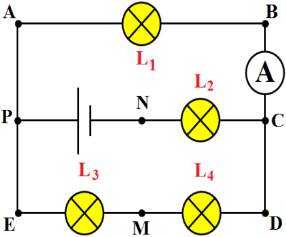
\includegraphics[width=0.28\textwidth]{./img/ex06.png}
  %\end{center}
%\end{wrapfigure}
	Le vinaigre commercial de degré d'acidité 6° est une solution de l'acide éthanoïque avec la formule
C2H4O2. Son degré d'acidité représente le pourcentage massique d'acide contenu dans la solution.
\begin{enumerate}
\item Déterminer la masse molaire de l'acide éthanoïque.
\item Calculer la concentration molaire des molécules d'acide éthanoïque dans ce vinaigre.
\end{enumerate}
Données: La masse volumique du vinaigre commercial: $\rho = 1,02 g/ml$.


\end{Box2}


\begin{Box2}{Exercice 7:Le degré alcoolique d’une boisson alcoolisée }
   % \begin{wrapfigure}[1]{r}{0.28\textwidth}
  %\begin{center}
	  %\vspace{-0.6cm}
	%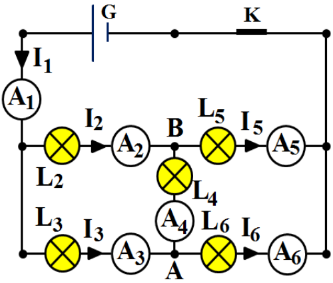
\includegraphics[width=0.28\textwidth]{./img/ex07.png}
  %\end{center}
%\end{wrapfigure}
	Le degré alcoolique d’une boisson alcoolisée représente le pourcentage volumique d’éthanol pur
contenu dans cette boisson.
\begin{enumerate}
\item Quel volume d’éthanol contient une bouteille de 75 cL d’un vin à 12°.
\item Quelle masse d’éthanol cela représente-t-il ?
\item En déduire la quantité de matière d’éthanol, puis la concentration en éthanol du vin.
\item Quel volume de vin doit-on prélever pour avoir $5,0.10^{-2}$ mol d’éthanol.
\end{enumerate}
Données: La densité de l’éthanol $C_2H_6O$: $d(C_2H_6O) = 0,79$.
\end{Box2}


\begin{center}
	\emph{If it weren't for electricity, we'd all be watching television by candlelight.}

	\emph{\textbf{Future Is Loading...}}

\end{center}

\end{document}
